\documentclass[10pt]{article}
\usepackage{femj_ru}
\usepackage{algorithm}% http://ctan.org/pkg/algorithms
\captionsetup[algorithm]{name=}
\usepackage[noend]{algpseudocode}
\usepackage{subfig}

\begin{document}
    \Pages(1--8)
    \def\Im{\mathop{\mathrm{Im}}\nolimits}
    \summary Mesenev~P.\,R., Chebotarev~A.\,Yu. \author
    Boundary inverse problem for conductive-radiative equations of heat transfer\title
    The boundary inverse problem of finding the reflecting properties of the boundary
    region for stationary radiation-conductive heat transfer equations in the
    three-dimensional region is considered. The existence of a quasi-solution of the
    inverse problem is proved and an optimality system is obtained. An algorithm for solving
    a problem is presented, the effectiveness of which is illustrated by numerical examples.
    \keywords{Radiative heat transfer equations, quasi-solution of the inverse problem,
        gradient descent method.}

    \UDC{517.95}
    \AMS{35K55, 35Q79}
    \SupportedBy{}
    \submitted{20 февраля 2018 г.}

    \title{Граничная обратная задача для уравнений сложного теплообмена}

    \author{П.\,Р.~Месенев}{Дальневосточный федеральный университет, 690950,
        г.~Владивосток, ул.~Суханова,~8;}{mesenev.pr@gmail.com}
    \author{А.\,Ю.~Чеботарев}{Институт прикладной математики ДВО РАН, 690041,
        Владивосток, ул. Радио, 7}{cheb@iam.dvo.ru}

    \makeface

    \abstract Рассмотрена граничная обратная задача нахождения отражающих
    свойств участка границы для стационарных уравнений радиационно-кондуктивного
    теплообмена в трёхмерной области.
    Доказано существование квазирешения обратной задачи и получена система оптимальности.
    Приведён алгоритм решения задачи, эффективность которого проиллюстрирована численными примерами.


    \keywords{уравнения радиационного теплообмена,
        квазирешение обратной задачи, метод градиентного спуска.}


    \section{Введение}
    Исследование математических моделей радиационного теплопереноса \cite{modest_rht},
    учитывающих одновременно вклад эффектов теплопроводности и излучения даёт теоретическую основу для инженерных решений в различных областях, таких как производство стекла \cite{OControl_3}, лазерная интерстициальная термотерапия \cite{tse_lasor}, и др. Главной особенностью данных процессов является существенное влияние излучения на теплообмен при высоких температурах. Значительное число работ посвящено исследованию задач управления для нестационарных моделей сложного теплообмена \cite{pinnau_identification, pinnau_optimal_control, pinnau_glass}, в которых для описания температурного поля используется нестационарное уравнение теплопроводности, а для моделирования излучения — стационарное диффузионное приближение уравнения переноса излучения. В работах \cite{covt_last, grenkin_13} задача оптимального управления сводится к bang-bang принципу \cite{grenkin_15}, или аналогичному. Близкие к рассмотренной в данной статье, задача управления коэффициентом отражения для полностью стационарной модели исследовалась в \cite{cheb_origin}, для нестационарной модели -- в \cite{grenkin_optimalnoe_upravleine}. Отметим также работы \cite{a6,a7}, в которых рассмотрены свойства квазирешений обратных задач для уравнений тепломассопереноса.

    Настоящая работа посвящена нахождению коэффициента отражения участка границы для стационарной модели, по дополнительной информации о температурном поле. Доказано существование квазирешения задачи. Предложен алгоритм градиентного спуска для решения экстремальной задачи и представлены результаты численных экспериментов.


    \section{Постановка обратной задачи}
    Нормализованная стационарная модель, описывающая процесс радиационного теплопереноса в области $\Omega \subset \mathbb{R}^3$ с липшицевой границей $\Gamma$ (см. \cite{OControl_1}), имеет следующий вид:
    \begin{equation}
        \label{initial}
        \begin{aligned}
            - a \Delta \theta + b \kappa_a(\theta ^ 3 | \theta | - \varphi) = 0,  \\
            - \alpha \Delta \varphi + \kappa_a (\varphi - \theta ^3 | \theta |) = 0.
        \end{aligned}
        % \qquad \text{в } \Omega.
    \end{equation}

    Здесь $\theta$ -- нормализованная температура, $\varphi$ -- нормализованная интенсивность излучения, усреднённая по всем направлениям, $\kappa_a$ -- коэффициент поглощения. Константы $a, b, \alpha, \gamma, \beta$ описываются следующим образом:
    \[
        a = \frac{k}{\rho c_v}, \; b = \frac{4 \sigma n^2 T^3_{\text{max}}}{\rho c_v}, \;
        \alpha = \frac{1}{3\kappa -A \kappa_s}
    \]
    где $k$ -- теплопроводность, $c_v$ -- удельная теплоёмкость, $\rho$ -- плотность, $\sigma$ -- постоянная Стефана\,--\,Больцмана, $n$ -- индекс рефракции, $T_{\text{max}}$ -- максимальная температура, $\kappa := \kappa_s + \kappa_a$ -- коэффициент полного взаимодействия, $\kappa_s$ -- коэффициент рассеяния. Коэффициент $A \in [-1,1]$ описывает анизотропию рассеивания; случай $A=0$ отвечает изотропному рассеиванию.

    Уравнения \eqref{initial} дополняются граничными условиями на $\Gamma := \partial \Omega =\overline{\Gamma}_0 \cup \overline{\Gamma}_1 \cup \overline{\Gamma}_2$, где части границы $\Gamma_0, \Gamma_1, \Gamma_2$ не имеют пересечений.

    \begin{equation}
        \label{initial-boundary}
        \begin{aligned}
            \Gamma &: \; a \partial_n \theta + \beta (\theta - \theta _b) = 0, \\
            \Gamma_0 \cup \Gamma_2 &: \; \alpha \partial_n \varphi + \gamma(\varphi - \theta_b ^4 ) = 0, \\
            \Gamma_1 &: \; \alpha \partial_n \varphi + u(\varphi - \theta_b ^4 ) = 0. \\
        \end{aligned}
    \end{equation}
    Функции $\gamma, \theta_b, \beta$ -- являются известными. Функция $u$ характеризует отражающие свойства участка границы $\Gamma_1$. Предполагается, что
    \begin{equation}
        \label{control_bounds}
        0 < u_1 \leq u \leq u_2,
    \end{equation}
    где $u_1$ и $u_2$ - заданные ограниченные функции.

    Обратная задача состоит в нахождении функций $u(x), x \in  \Gamma_1, \; \theta(x), \varphi(x), x \in \Omega $ удовлетворяющих условиям \eqref{initial}--\eqref{control_bounds}, а также дополнительному условию на участке границы $\Gamma_2$:
    \begin{equation}
        \label{theta_gamma}
        \theta|_{\Gamma_2}=\theta_0
    \end{equation}
    где $\theta_0$ известная функция.
    Сформулированная обратная задача \eqref{initial}--\eqref{theta_gamma} сводится к экстремальной задаче, состоящей в минимизации функционала
    \begin{equation}
        \label{quality}
        J(\theta) = \frac{1}{2} \int_{\Gamma_2} (\theta - \theta_0)^2 d\Gamma
    \end{equation}
    на решениях краевой задачи \eqref{initial}--\eqref{control_bounds}.
    Решение задачи \eqref{initial}--\eqref{control_bounds}, \eqref{quality} называется квазирешением задачи \eqref{initial}--\eqref{theta_gamma}

    %\section{������������ ������ ���������� ������������}

����� ������������ ��� �������� ������ ������������� ���������� �������:

(i) $\beta, \gamma \in L^\infty(\Gamma); u_1, u_2 \in L^\infty(\Gamma_1); 0 < \gamma_0 \le \gamma; \; 0 \le u_1 \le u_2;$

����� $H = L^2(\Omega), V = W^1_2(\Omega), Y = V \times V $. ������������ $H$ ������������� � ������������� $H'$ ���,  ��� $V \subset H = H' \subset V'$. ��������� $(f,v)$ ��� �������� ����������� $f \in V'$ �� �������� $v \in V$, ����������� �� ��������� ������������� � $H$, ���� $f\in H, \|f\|^2 = (f,f)$. ������������ $U = L^2(\Gamma_1)$ �������� ������������� ����������. ��������� ���������� ����������: $U_{ad} = \{u \in U, u_1 \le u \le u_2 \}$.

����� $v$ ������������ ������� ��������� $H^1(\Omega)$. ��������� ��������� ���������:

$$A_{1,2}\colon V \to V', \;\; F \colon V \times U \to V', \; f \in V', \; g \in V'.$$
$$(A_1\theta,v) = a( \nabla \theta, \nabla v ) + \int_\Gamma \beta \theta v d\Gamma, \;
(A_2 \varphi, v) = \alpha (\nabla \varphi,\nabla v) + \int_{\Gamma_0 \cup \Gamma_2} \gamma \varphi v d\Gamma,$$
$$(f,v) = \int_\Gamma \beta \theta_b v d\Gamma, \; \;
(g,v) = \int_{\Gamma_0 \cup \Gamma_2} \gamma \theta_b^4 v d\Gamma,$$
$$(F(\varphi, u), v) = \int_{\Gamma_1} u (\varphi - \theta^4_b)v d\Gamma.$$

���� $\{\theta, \varphi \} \in Y$ ����� �������� ������ �������� ������ \eqref{initial}, \eqref{initial_boundary}, ����
\begin{equation}
    \label{weak_operational}
    A_1 \theta + b \kappa_a (| \theta | \theta^3 - \varphi ) = f, A_2 \varphi + \kappa_a (\varphi - |\theta|\theta^3) + F(\varphi, u) = g.
\end{equation}

������ ���������� ������������ ������� � ����������� ����������� $J(\theta)$, ������������ �� ���������� $\theta$ ������� ������� \eqref{weak_operational}. ����� �������
    \begin{equation}
        \label{minimization_operational}
        J(\theta, u) \to \text{inf}, \; \{\theta, \varphi\} \text{ ������� \eqref{weak_operational},   ��������������  ������� } u \in U_{ad}.
    \end{equation}

    ���� $\{\hat{\theta}, \hat{\varphi} \}$ ��������������� �������� $J$, ���������� ������� $\hat{u}$ ���������� ����������� ����������. � ����� ������ $\hat{u}$ ���������� ������������� �������� ������ \eqref{initial}--\eqref{theta_gamma}.



    \section{Формализация задачи нахождения квазирешения}

    Будем предполагать что исходные данные удовлетворяют следующему условию:

    (i) $\beta\in L^\infty(\Gamma);\; \gamma \in L^\infty(\Gamma_0\cup\Gamma_2);\; u_1, u_2 \in L^\infty(\Gamma_1);
    \; 0 < \beta_0 \le \beta;\;  0 < \gamma_0 \le \gamma; \; \beta_0,\gamma_0=Const,\;\;\\ 0 \le u_1 \le u_2;$

    Пусть $H = L^2(\Omega), V = W^1_2(\Omega), Y = V \times V $. Пространство $H$ отождествляем с сопряжённым пространством $H'$ так, что $V \subset H = H' \subset V'$. Определим $(f,v)$ как значение функционала $f \in V'$ на элементе $v \in V$, совпадающее со скалярным произведением в $H$, если $f\in H, \|f\|^2 = (f,f)$. Пространство $U = L^2(\Gamma_1)$ является пространством управлений;
    $U_{ad} = \{u \in U, u_1 \le u \le u_2 \}$ --- множество допустимых управлений.

    Пусть $v$ произвольный элемент множества $H^1(\Omega)$. Определим операторы:

    $$A_{1,2}\colon V \to V', \;\; F \colon V \times U \to V', \; f \in V', \; g \in V'.$$
    $$(A_1\theta,v) = a( \nabla \theta, \nabla v ) + \int_\Gamma \beta \theta v d\Gamma, \;
    (A_2 \varphi, v) = \alpha (\nabla \varphi,\nabla v) + \int_{\Gamma_0 \cup \Gamma_2} \gamma \varphi v d\Gamma,$$
    $$(f,v) = \int_\Gamma \beta \theta_b v d\Gamma, \; \;
    (g,v) = \int_{\Gamma_0 \cup \Gamma_2} \gamma \theta_b^4 v d\Gamma,$$
    $$(F(\varphi, u), v) = \int_{\Gamma_1} u (\varphi - \theta^4_b)v d\Gamma.$$

    Пару $\{\theta, \varphi \} \in Y$ будем называть слабым решением задачи \eqref{initial}, \eqref{initial-boundary}, если
    \begin{equation}
        \label{weak_operational}
        A_1 \theta + b \kappa_a (| \theta | \theta^3 - \varphi ) = f, A_2 \varphi + \kappa_a (\varphi - |\theta|\theta^3) + F(\varphi, u) = g.
    \end{equation}

    Задача нахождения квазирешения состоит в минимизации функционала $J(\theta)$, определённом на компоненте $\theta$ решения системы \eqref{weak_operational}. Таким образом
    \begin{equation}
        \label{minimization_operational}
        J(\theta) \to \text{inf}, \; \{\theta, \varphi\} \text{ решение \eqref{weak_operational}, соответствующее функции } u \in U_{ad}.
    \end{equation}

    Пара $\{\hat{\theta}, \hat{\varphi} \}$ соответствующая минимуму $J$, отвечающая функции $\hat{u}$ называется оптимальным состоянием. В таком случае $\hat{u}$ называется квазирешением обратной задачи \eqref{initial}--\eqref{theta_gamma}.

    %\section{������ ������������� ������}
\label{sec:optimality}

��� �������������� ������������ ������ \eqref{minimization_operational} ��� ���������� ����� ���������� ��������� �������� ������� ������ \eqref{initial}, \eqref{initial_boundary}.

\begin{lem}[\cite{lemma_proof}]

\label{SolvabilityLemma}

    ���� ������� (i) �����������, �� ��� ������� $ u \in U_{ad} $ ���������� ������������ ������ ������� $\{\theta, \varphi \}$ ��� ������ \eqref{initial},\eqref{initial_boundary}, ����� ����� ��������� ������:
    \begin{equation}
        \label{lemma_1}
     M_1 \le \theta \le M_2, \; M_1^4 \le \varphi \le M_2^4,
     \end{equation}

    \begin{equation}
    \label{lemma_2}
     \| \nabla \varphi \|^2 \le C.
     \end{equation}
    ����� $M_1 = \text{ess inf } \theta_b, M_2 = \text{ess sup } \theta_b$, � ��������� $C > 0$ ������� ������ �� \\ $a, b, \alpha, \kappa_a, \|u\|_{L^\infty(\Gamma)}, \| \gamma \|_{L^\infty(\Gamma)}$ � ������� $\Omega$.
\end{lem}

�� ������ ������ \eqref{lemma_1} � \eqref{lemma_2} ������������ ������������ ������������� ������ \eqref{minimization_operational}.
\begin{thm}[��. \cite{cheb_origin}]
    ���� ������� (i) �����������, ����� ���������� ���� �� ���� ������� ������ \eqref{minimization_operational}.
\end{thm}


��� ������ ������� �������������, ������� ������������������ ����������� $J$.
\begin{lem}
\label{freshet_diff}
    ���������� $J : V \rightarrow \mathbb{R}$ �������������� �� �����.
\end{lem}

\begin{proof}
�������, ��� ��� ������������ ������� $\theta \in V$ ����������� ��������� ���������:

\begin{equation}
\label{lemma_proof_1}
J(\theta + h) = J(\theta) + J'(\theta)\langle h \rangle + r(\theta, h) \; \forall h \in V, \; \text{ ��� } \; J'(\theta)\langle h \rangle = \int_{\Gamma_2} (\theta - \theta_0)h d\Gamma
\end{equation}

��� ��� ����������� ����� $r(\theta,h)$ ����������� �����������:
\begin{equation}
\label{lemma_proof_2} \frac{1}{2} \frac{|r(\theta,h)|}{\|h\|_V} \rightarrow 0 \quad \text{���} \quad \|h\|_V \rightarrow 0.
\end{equation}


��������� \eqref{lemma_proof_1} � ����

$$
    \frac{1}{2} \|\theta + h - \theta_0\|^2_{L^2(\Gamma_2)} =
    \frac{1}{2} \| \theta - \theta_0 \|^2_{L^2(\Gamma_2)} +
    (\theta - \theta_0, h)_{L^2(\Gamma_2)} +
    \frac{1}{2}\| h \|^2_{L^2(\Gamma_2)}.
$$



�������� ������� � ������ \cite{alekseev_monograph} $ \|h\|_{L^2(\Gamma_2)} \le C \|h\|_V $, ��� $C$ �� ������� �� $h$. �������
$$
\frac{1}{2}
\frac{r(\theta,h)}{\| h \|_V} \leq
\frac{1}{2} C^2 \| h \|_V \rightarrow 0 \quad \text{��� } \| h \|_V \rightarrow 0.
$$

\end{proof}

����� ������� ������������� ������� �� �������� ���������� �������� ��� ������-�������� ����� �����������.
\begin{thm}
\label{adjoint_theorem}
    ����� $\hat{y}=\{\hat{\theta},\hat{\varphi} \} \in Y, \hat{u} \in U_{ad}$ �������  ������������� ������ \eqref{minimization_operational}. ����� ���������� ���� $p = (p_1, p_2), p \in \mathbb{R}_{+} \times Y \setminus \{0\}$
    �����, ��� ������ $(\hat{y}, \hat{u}, p)$, ������������� ��������� ��������:
    \begin{equation}
        \label{therorem_2_eq1}
         A_1 p_1 + 4 |\hat{\theta}|^3 \kappa_a(b p_1 - p_2) = f_c, \;\; (f_c,v) = - \int_{\Gamma_2} (\hat{\theta} - \theta_0) v d\Gamma,
    \end{equation}

    \begin{equation}
        \label{therorem_2_eq2}
        A_2 p_2 + \kappa_a (p_2-b p_1) = g_c(( p_2, \hat{u}),v), \;\; g_c(( p_2, \hat{u}),v) = -\int_{\Gamma_1} \hat{u} p_2 v\Gamma,
    \end{equation}

    \begin{equation}
        \label{therorem_2_eq3}
        \int_{\Gamma_1} p_2 (\hat{\varphi} - \theta_b^4)(u-w) \leq 0 \quad \forall w \in U_{ad}.
    \end{equation}
\end{thm}
\begin{proof}
    ��������� ��������� \eqref{weak_operational} ��������� �������:
    $$H(y,u) = 0,\;\; y = \{\theta,\varphi\} \in Y,$$
    ���
    $$ H:Y \times U \to Y', $$
    $$H(y,u) =\{A_1 \theta + b \kappa_a (| \theta | \theta^3 - \varphi ) - f, A_2 \varphi + \kappa_a (\varphi - |\theta|\theta^3) + F(\varphi, u) - g \}.$$
    �������, ��� ��� ���� $u \in U_{ad}$, ����������� $y \to J(\theta) $ � $y \to H(y,u)$ ���������� ��������������� � ����������� $\mathcal{O}(\hat{y})$ ����� $\hat{y}$. ����������� ������������������ ������ � $H$ ������� �� ����������� ������������������ ������� $t \in \mathbb{R} \to | t | t^3$, � ����� �� ������������� ��������  $V \subset L^6(\Omega)$.
    � ����������, ����������� $u \to H(y,u)$ ���������� �� $U \to Y'$ � ������.

    � \cite{theorem_2_proof} ��������, ��� $\text{Im}H_y'(\hat{y}, \hat{u}) = Y$, ��� ������ ��������������� ������� �������������.
    
    ���������� ������� ��������
    $L(y,u,p) = J(\theta) + (H(y,u),p),$
    ��� $y,p \in Y,\, u \in U_{ad}$. �������� �������� �������� \cite[��.2, ������� 1.5]{theorem_proof_18} ���������� ���� $p = \{p_1,p_2\} \in Y$ �����, ���

    \begin{equation}
        \label{th2_proof_1}
        (L_\theta,\zeta) =\int_{\Gamma_2}(\hat\theta -\theta_0) \zeta d\Gamma + (A_1 \zeta + 4b\kappa_a |\hat\theta|^3 \zeta,p_1) - 4\kappa_a(|\hat\theta|^3 \zeta,p_2) = 0 \; \forall \zeta \in V,
    \end{equation}

    \begin{equation}
        \label{th2_proof_2}
        (L_\varphi, \zeta) = (A_2 \zeta + \kappa_a \zeta, p_2) - b \kappa_a(\zeta,p_1) +\int_{\Gamma_1} \hat u \zeta p_2 = 0 \; \forall \zeta \in V,
    \end{equation}

    \begin{equation}
        \label{th2_proof_3}
        (L_u,\tau) = \int_{\Gamma_1} \tau (\varphi - \theta^4_b) p_2 d\Gamma  \leq 0, \; \tau := \hat u - w \; \forall w \in U_{ad}.
    \end{equation}

    ����������� ��������� �������� ������ ���������� \eqref{th2_proof_1} � \eqref{th2_proof_2}.

\end{proof}

% ���������: ������ �� �����, ��� ��� ImH'_y =  Y'

% ��� �������������� ��������� �������, ��� ����������� �����
% \begin{lem}[����� 2 � \cite{covt_last}]
%     ����� $h > 0$ ��������� ������� �� $L^\infty(\Omega)$. ���� ������� $q_1,q_2 \in V$ ������������� ����������
%     \begin{equation}
%     \label{lemma_eq_for_theorem}
%         A_1q_1 +b \kappa_a(hq_1 - q_2) = 0, A2q_2 + F(q_2,\hat{u}) + \kappa_a(q_2 - h q_1) = 0,
%     \end{equation}
%     ����� $q_1 = q_2 = 0$.
% \end{lem}

% ������, �������� �� ����������� ����� �� ����� �������� ��������� �������
% \begin{theorem}[������� 3 � \cite{covt_last}]

%     ����� $\hat{y} = \{\hat{\theta}, \hat{\varphi}\} \in Y$, $\hat{u} \in U_{ad}$ ����� �������� ������ ������������ ���������� \eqref{minimization_operational}. ����� ���������� ���� $p = \{p_1,p_2\} \in Y$ �����, ��� ������ �������� $(y, u, p)$ ������������� ������� ���������
%     \begin{equation}
%         A_1 p_1 + 4 \hat{\theta}^3 \kappa_a(b p_1 - p_2) = f_c, \;\;
%         f_c = - (\theta - \theta_0) \; \text{ �� } \; \Gamma_2,
%     \end{equation}

%     \begin{equation}
%         A_2 p_2 + \kappa_a (p_2-b p_1) = g_c( p_2, \hat{u}),
%         \;\; g_c(p_2,\hat{u}) = - u p_2 \; \text{ �� } \; \Gamma_1,
%     \end{equation}

%     \begin{equation}
%         \int_{\Gamma_1} p_2 (\hat{\varphi} - \theta_b^4)(w - u) d\Gamma \ge 0, \; \; \forall w \in U_{ad}.
%     \end{equation}
% \end{theorem}
% \begin{proof}
% �����������, ��� ��������� $\lambda$ ����� ���� ��� ������������ $f_c$ � $g_c(p_2,\hat{u})$ � ���������� \eqref{therorem_2_eq1} � \eqref{therorem_2_eq2}. ������� �����, �� ����� ������������� ������� ��������� $p = 0$, ���, � ���� �������, ������������ �������  \ref{adjoint_theorem} �, ��� �����, ��������� ���������� ��������������� $\lambda$ � ��������� �������� ��������� $\lambda$ ������ $1$.

% ��� ����� ��������� �������� \eqref{therorem_2_eq1} � \eqref{therorem_2_eq2} � ����������� ���� � ������������ $Y = V \times V$, �� �������� �������������:
% $$
%     (y,z)_Y = (A_1,y_1,z_1) + (A_2 y_2 + F(y_2, \hat{u}), z_2), \;\; y=\{y_1,y_2\}, z = \{z_1,z_2\}
% $$
% ��������� �������� $R: Y \rightarrow Y$ ���
% $$
%     Rp = \{A_1^{-1} (4 \hat{\theta}^3 \kappa_a (b p_1 - p_2)), \kappa_a A^{-1}_2(p_2 -b p_1) \},
% $$
% ����� ������� ��������� \eqref{therorem_2_eq1} � \eqref{therorem_2_eq2} ��� $\lambda = 0$ ������������ ���������
% \begin{equation}
% \label{fredholm_type}
%     p + Rp = 0 \, \text{�} \; Y
% \end{equation}
% �������, ��� �������� $R$ �������� ����������. �������������, ��������� ��������� ����� ��� ���� $\nu =\{\nu_1, \nu_2\} \in Y$
% $$
%     (R_p,\nu)_Y = (4 \hat{\theta}^3 \kappa_a (b p_1 - p_2), \nu_1) + \kappa_a(p_2 - b p_1, \nu_2) \leq
%     C(\| p_1 \| + \| p_2 \|) \| \nu \|_Y,
% $$
% ��� ��������� $C > 0$ �� ������� �� $p$ � $\nu$.
% ����� �������, ���� �� ������� $\nu = Rp$ �� ������� ��������� ������
% $$
%     \|Rp\|_Y \le C(\|p_1\|+\|p_2\|).
% $$
% ������������ ��������� $R$ ������� �� ������������ �������� $V \subset H$. ����� ������� ����������� ������������ ��������� ���������� \eqref{fredholm_type} ������� �� ������� $Ker(I+R*) = \{0\}$. ���, ������� �������, ��������� $q + R*q =0$ ������ ����� ������ ����������� �������. ������� ������, ��� ��������� ��������� ������������ ������� ��������� \eqref{lemma_eq_for_theorem}
%     % TODO: ����� �� ������ ��������� �� [lemma 2]{covt_last}
% \end{proof}



    \section{Анализ экстремальной задачи}
    \label{sec:optimality}

    Для доказательства разрешимости задачи~\eqref{minimization_operational} нам необходимо также установить некоторые свойства решения задачи \eqref{initial}, \eqref{initial-boundary}.

    \begin{lem}[\cite{lemma_proof}]
        \label{SolvabilityLemma}
        Пусть выполняется условие (i). Тогда для каждого $ u \in U_{ad} $ существует единственное слабое решение $\{\theta, \varphi \}$ для задачи \eqref{initial},\eqref{initial-boundary} и справедливы оценки:
        \begin{equation}
            \label{lemma_1}
            M_1 \le \theta \le M_2, \; M_1^4 \le \varphi \le M_2^4,
        \end{equation}
        \begin{equation}
            \label{lemma_2}
            \| \nabla \varphi \|^2 \le C.
        \end{equation}
        Здесь $M_1 = \text{ess inf } \theta_b, M_2 = \text{ess sup } \theta_b$, и константа $C > 0$ зависит только от \\ $a, b, \alpha, \kappa_a, \beta, \gamma, \|u\|_{L^\infty(\Gamma)}$ и области $\Omega$.
    \end{lem}

    На основе оценок \eqref{lemma_1} и \eqref{lemma_2} аналогично \cite{cheb_origin} доказывается разрешимость экстремальной задачи \eqref{minimization_operational}.
    \begin{thm}
        Пусть выполняется условие (i). Тогда существует хотя бы одно решение задачи \eqref{minimization_operational}.
    \end{thm}


    Для вывода системы оптимальности, покажем дифференцируемость функционала $J$.
    \begin{lem}
        \label{freshet_diff}
        Функционал $J : V \rightarrow \mathbb{R}$ дифференцируем по Фреше.
    \end{lem}
    \begin{proof}
        Покажем, что для произвольной функции $\theta \in V$ выполняется следующее равенство:
        \begin{equation}
            \label{lemma_proof_1}
            J(\theta + h) = J(\theta) + J'(\theta)\langle h \rangle + r(\theta, h) \; \forall h \in V, \; \text{ где } \; J'(\theta)\langle h \rangle = \int_{\Gamma_2} (\theta - \theta_0)h d\Gamma,
        \end{equation}
        где для остаточного члена $r(\theta,h)$ справедливо соотношение:
        \begin{equation}
            \label{lemma_proof_2} \frac{|r(\theta,h)|}{\|h\|_V} \rightarrow 0 \quad \text{при} \quad \|h\|_V \rightarrow 0.
        \end{equation}
        Перепишем \eqref{lemma_proof_1} в виде
        $$
        \frac{1}{2} \|\theta + h - \theta_0\|^2_{L^2(\Gamma_2)} =
        \frac{1}{2} \| \theta - \theta_0 \|^2_{L^2(\Gamma_2)} +
        (\theta - \theta_0, h)_{L^2(\Gamma_2)} +
        \frac{1}{2}\| h \|^2_{L^2(\Gamma_2)}.
        $$
        Согласно теореме о следах $ \|h\|_{L^2(\Gamma_2)} \le C \|h\|_V $, где $C$ не зависит от $h$. Поэтому
        $$
        \frac{r(\theta,h)}{\| h \|_V} \leq
        \frac{1}{2} C^2 \| h \|_V \rightarrow 0 \quad \text{при } \| h \|_V \rightarrow 0.
        $$
    \end{proof}

    Вывод условий оптимальности основан на принципе множителей Лагранжа для гладко-выпуклых задач минимизации.
    \begin{thm}
        \label{adjoint_theorem}
        Пусть $\hat{y}=\{\hat{\theta},\hat{\varphi} \} \in Y, \hat{u} \in U_{ad}$ --- решение экстремальной задачи \eqref{minimization_operational}. Тогда существует пара $p = (p_1, p_2)$, $p \in Y$
        такая, что тройка $(\hat{y}, \hat{u}, p)$, удовлетворяет следующим условиям:
        \begin{equation}
            \label{therorem_2_eq1}
            A_1 p_1 + 4 |\hat{\theta}|^3 \kappa_a(b p_1 - p_2) = f_c, \;\; (f_c,v) = - \int_{\Gamma_2} (\hat{\theta} - \theta_0) v d\Gamma,
        \end{equation}
        \begin{equation}
            \label{therorem_2_eq2}
            A_2 p_2 + \kappa_a (p_2-b p_1) = g_c(( p_2, \hat{u}),v), \;\; g_c(( p_2, \hat{u}),v) = -\int_{\Gamma_1} \hat{u} p_2 v\Gamma,
        \end{equation}
        \begin{equation}
            \label{therorem_2_eq3}
            \int_{\Gamma_1} p_2 (\hat{\varphi} - \theta_b^4)(u-w) \leq 0 \quad \forall w \in U_{ad}.
        \end{equation}
    \end{thm}
    \begin{proof}
        Перепишем уравнения \eqref{weak_operational} следующим образом:
        $$H(y,u) = 0,\;\; y = \{\theta,\varphi\} \in Y,$$
        где
        $$ H:Y \times U \to Y', $$
        $$H(y,u) =\{A_1 \theta + b \kappa_a (| \theta | \theta^3 - \varphi ) - f, A_2 \varphi + \kappa_a (\varphi - |\theta|\theta^3) + F(\varphi, u) - g \}.$$
        Заметим, что для всех $u \in U_{ad}$, отображение $y \to J(\theta) $ и $y \to H(y,u)$ непрерывно дифференцируемо в окрестности $\mathcal{O}(\hat{y})$ точки $\hat{y}$. Непрерывная дифференцируемость членов в $H$ следует из непрерывной дифференцируемости функции $t \in \mathbb{R} \to | t | t^3$, а также из непрерывности вложения  $V \subset L^6(\Omega)$.
        В дополнение, отображение $u \to H(y,u)$ непрерывно из $U \to Y'$ и афинно.
        В \cite{cheb_origin} показано, что $\text{Im}H_y'(\hat{y}, \hat{u}) = Y$, что влечёт невырожденность условий оптимальности.

        Рассмотрим функцию Лагранжа
        $L(y,u,p) = J(\theta) + (H(y,u),p),$
        где $y,p \in Y,\, u \in U_{ad}$. Согласно принципу Лагранжа \cite[Гл.2, Теорема 1.5]{theorem_proof_18} существует пара $p = \{p_1,p_2\} \in Y$ такая, что
        \begin{equation}
            \label{th2_proof_1}
            (L_\theta,\zeta) =\int_{\Gamma_2}(\hat\theta -\theta_0) \zeta d\Gamma + (A_1 \zeta + 4b\kappa_a |\hat\theta|^3 \zeta,p_1) - 4\kappa_a(|\hat\theta|^3 \zeta,p_2) = 0 \; \forall \zeta \in V,
        \end{equation}
        \begin{equation}
            \label{th2_proof_2}
            (L_\varphi, \zeta) = (A_2 \zeta + \kappa_a \zeta, p_2) - b \kappa_a(\zeta,p_1) +\int_{\Gamma_1} \hat u \zeta p_2 = 0 \; \forall \zeta \in V,
        \end{equation}
        \begin{equation}
            \label{th2_proof_3}
            (L_u,\tau) = \int_{\Gamma_1} \tau (\varphi - \theta^4_b) p_2 d\Gamma  \leq 0, \; \tau := \hat u - w \; \forall w \in U_{ad}.
        \end{equation}
        Сопряжённые уравнения \eqref{therorem_2_eq1},\eqref{therorem_2_eq2} являются прямым следствием
        вариационных равенств \eqref{th2_proof_1} и \eqref{th2_proof_2}.
    \end{proof}


    \section{Численные эксперименты}
    Пусть функционал $J(\theta)$ удовлетворяет условиям, указанным в \autoref{sec:optimality}. Для удобства введём переобозначение $\hat{J}(u):=J(\theta(u)), \hat{J}:L^2(\Gamma_1) \to \mathbb{R}$. Здесь $\theta(u)$ -- температурное поле задачи  \eqref{initial}--\eqref{initial-boundary} отвечающее управлению $u \in L^2(\Gamma_1)$.
    Согласно формуле \eqref{therorem_2_eq3} градиент функционала $\hat{J}(u)$ \cite{grenkin_13} имеет вид
    $$\hat{J}'(u)= (\varphi(u) -\theta_b^4)p_2,$$
    где $\varphi(u)$ есть интенсивность излучения, $p_2$ -- соответствующая переменная сопряжённой системы.

    Предлагаемый алгоритм решения выглядит следующим образом:
    \begin{algorithm}[H]
        \caption{Алгоритм градиентного спуска с проекцией}
        \begin{algorithmic}[1]
            \State Выбираем значение градиентного шага $\lambda$,
            \State Выбираем количество итераций $N$,
            \State Выбираем произвольное $u_0 \in U_{ad}$,
            \For{$k \gets 0,1,2,...,N$}
                :
                \State Для полученного $u_k$ расчитываем состояние $y_k = \{\theta_k, \varphi_k\}$ из  (\ref{weak_operational}).
                \State Расчитываем значение функционала качества $J(\theta_k)$ из (\ref{quality}).
                \State Расчитываем сопряжённое состояние $p_k=\{p_{1k},p_{2k}\}$ из уравнений \eqref{therorem_2_eq1}--\eqref{therorem_2_eq2}, где $ \hat{\theta} := \theta_k, \hat{u}=u_k$.
                \State Пересчитываем управление $u_{k+1} = P_{ad}\left[ u_k - \lambda (\varphi_k - \theta_b^4)p_{2k} \right]$.
            \EndFor
        \end{algorithmic}
    \end{algorithm}
    Оператор проекции $P_{ad} : U \to U_{ad}$ определён следующим образом
    \[
        P_{ad}[v] =
        \begin{cases}
            u_1, & \text{если } v \le u_1 \\
            v, & \text{если } u_1 < v < u_2 \\
            u_2, & \text{если } v \ge u_2
        \end{cases}
    \]
    Приведём далее примеры расчётов для двумерного случая.
    Положим $\Omega = \{(x,y), 0 \leq x,y \leq 1\}$, $l = 1$ см.
    Граница $\partial\Omega$ состоит из участков:
    \[
        \begin{aligned}
            \Gamma_0 & = \{x=\{0,1\}, y \in [0,1]\} \\
            \Gamma_1 & = \{x\in [0,1], y=0\} - \text{участок с неизвестными отражающими свойствами,} \\
            \Gamma_2 & = \{x \in [0,1], y=1\} - \text{участок наблюдения.}
        \end{aligned}
    \]
    Будем также далее считать, что $a = 0.006[\text{см}^2/\text{c}]$, $b=0.025[\text{см}/\text{с}]$, $\beta = 0.00005[\text{см}/\text{с}]$, $\kappa=1[\text{см}^{-1}]$, $\kappa_s = 0$, $A = 0$, $\gamma = 0.3$. Указанные параметры соответствуют стеклу \cite{grenkin_13}.
    Температуру на границе $\Omega$ положим равной $\theta_b = (x^2+y^2)/3$.

    При указанных параметрах для первого эксперимента выберем следующее тестовое значение
    функции $u$ (рис. \ref{control}\subref{fig1:exp1}):
    \begin{equation}
        u(x)=
        \begin{cases}
            0.01, & \text{если } x \le 0.5, \\
            0.5, & \text{если } x > 0.5,
        \end{cases}
    \end{equation}
    и для второго эксперимента (рис. \ref{control}\subref{fig1:exp2}):
    \begin{equation}
        \label{test_function_1}
        u(x)=0.49x+0.01. \;
    \end{equation}

    Вычислим решение прямой задачи \eqref{initial}--\eqref{initial-boundary} для этих случаев. Полученное температурное поле на участке наблюдения $\Gamma_2$ выберем в качестве $\theta_0$. Далее, применяя предложенный алгоритм находим квазирешение обратной задачи \eqref{initial}--\eqref{theta_gamma}. Эффективность алгоритма, а также значение $u_0$ в первом и втором случаях иллюстрируются рис. \ref{control}. На рис. \ref{cost} показана динамика функционала качества по итерациям.

        {\bf Замечание.} В предложенных примерах потребовалось $2*10^6$ итераций для нахождения квазирешения $u$. В то же время температурное поле на участке наблюдения $\Gamma_2$ становится близким к $\theta_0$ уже на $10^2$ итерации. Также наблюдается существенное падение скорости уменьшения функционала качества с каждой итерацией после того, как среднее значение найденной функции контроля становится близко к тестовой функции.
    \begin{figure}[H]
        \centering
        \subfloat[Первый эксперимент]
        {
            \label{fig1:exp1}
            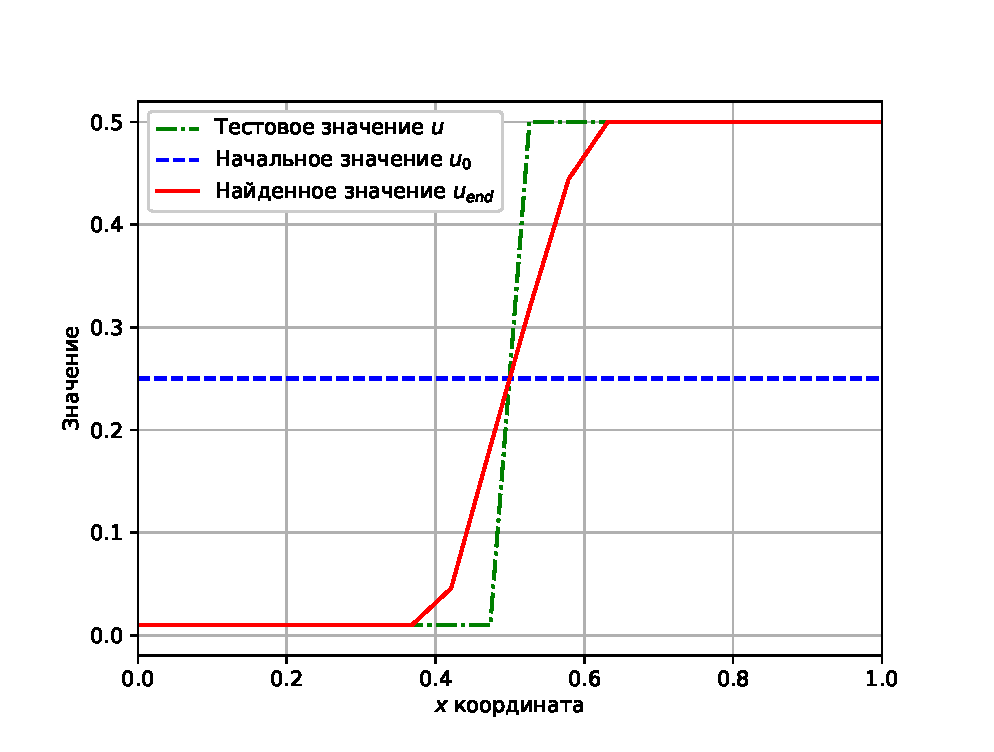
\includegraphics[width=.51\linewidth]{1.eps}
        }
        \subfloat[Второй эксперимент]
        {
            \label{fig1:exp2}
            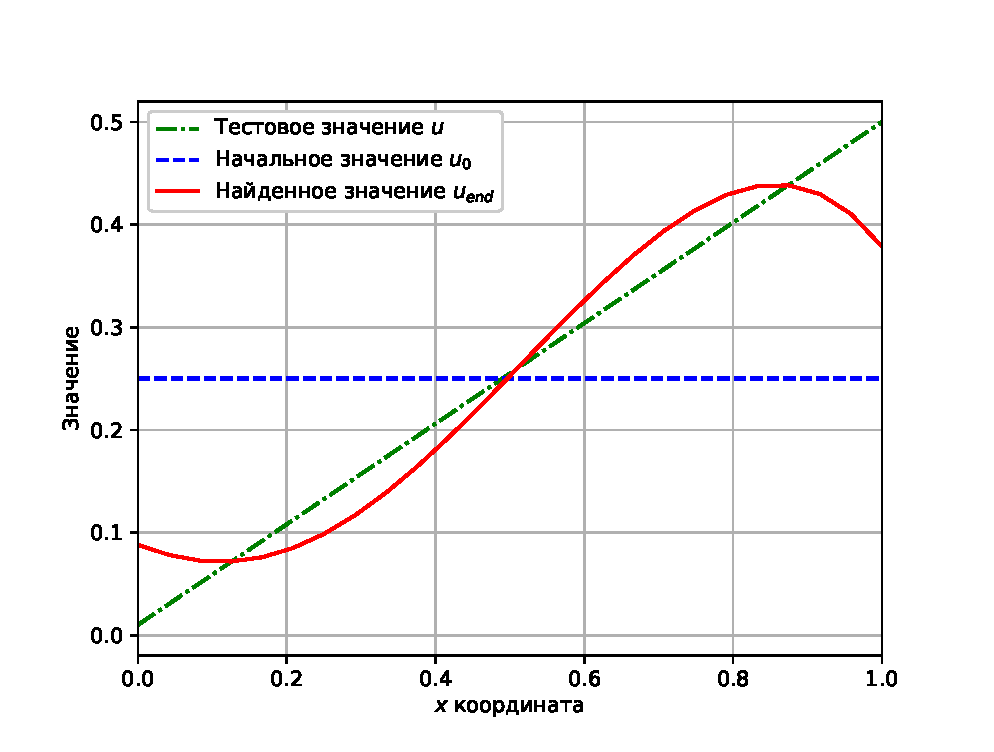
\includegraphics[width=.51\linewidth]{2.eps}
        }
        \caption{Тестовая функция $u$, начальная $u_0$, найденная функция $u_{end}.$}
        \label{control}
    \end{figure}

    \begin{figure}[H]
        \centering
        \subfloat[Первый эксперимент]
        {
            \label{fig2:exp1}
            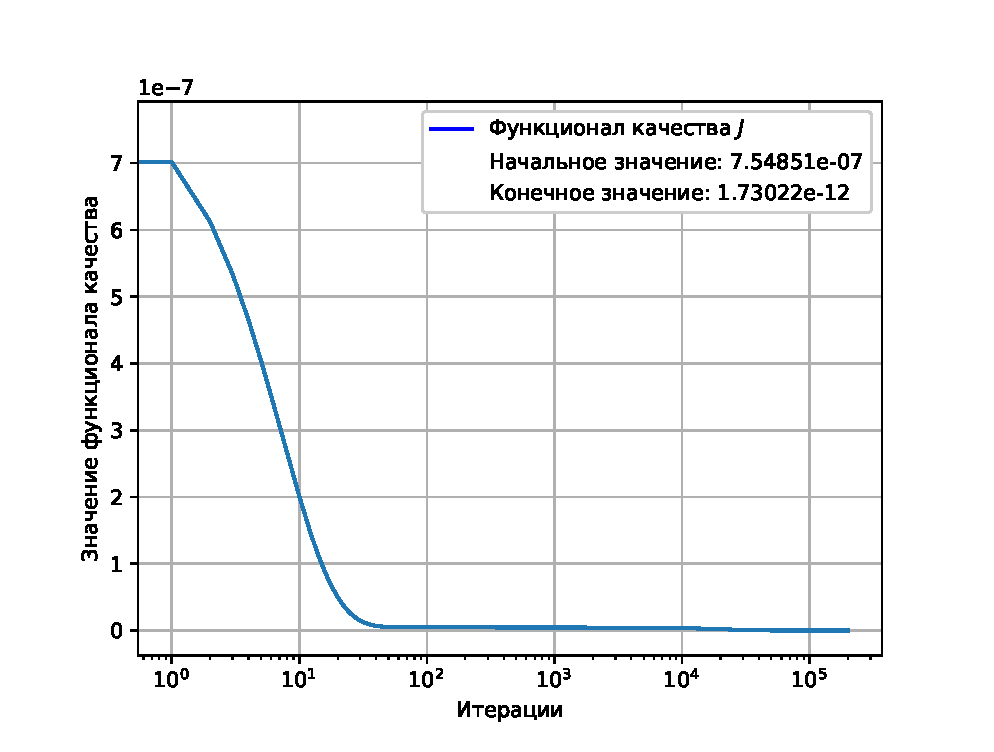
\includegraphics[width=.51\linewidth]{3.eps}
        }
        \subfloat[Второй эксперимент]
        {
            \label{fig2:exp2}
            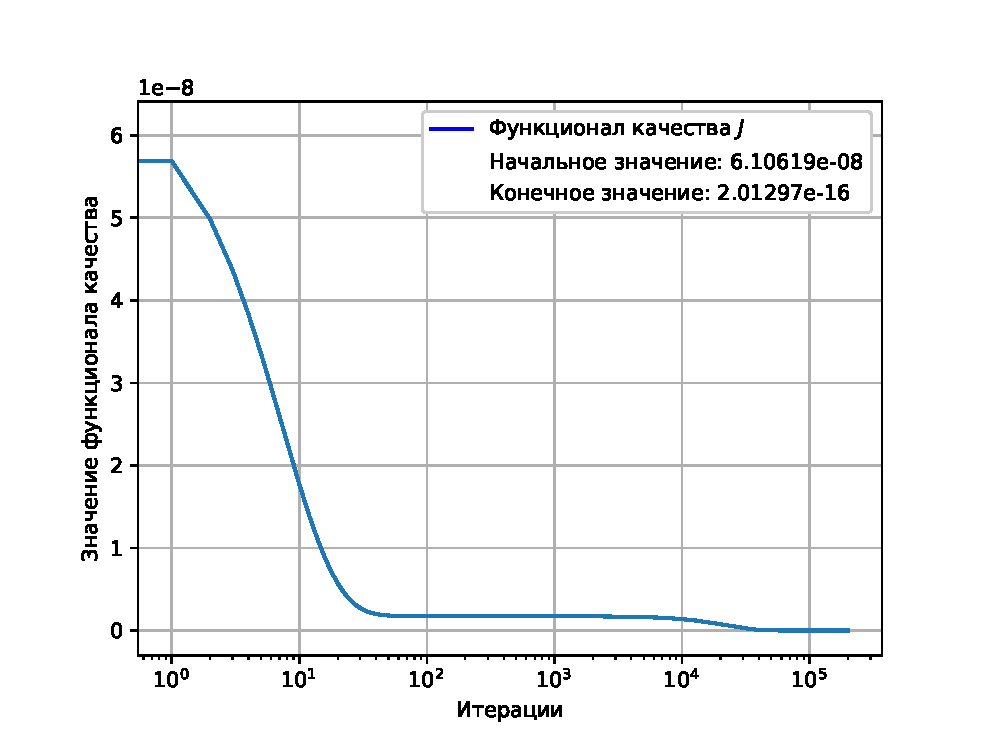
\includegraphics[width=.51\linewidth]{4.eps}
        }
        \caption{Динамика функции $\hat{J}(u)$ по итерациям.}
        \label{cost}
    \end{figure}

    \begin{thebibliography}{10}

        \Bibitem{modest_rht}
        \by M.\,F.~Modest
        \book Radiative Heat Transfer
        \publ Academic Press
        \yr 2003

        \Bibitem{OControl_3}
        \vol 33
        \issue 2
        \pages 157--175
        \yr 2012
        \by Clever D. and Lang J.
        \paper Optimal control of radiative heat transfer in glass cooling with restrictions on the temperature gradient

        \Bibitem{tse_lasor}
        \by O.~Tse, R.~Pinnau, N.~Siedow
        \paper Identification of temperature dependent parameters in laser--interstitial thermo therapy
        \jour Math. Models Methods Appl. Sci.
        \vol 22
        \issue 9
        \yr 2012
        \pages 1--29O

        \Bibitem{pinnau_identification}
        \by N.~Siedow O.~Tse, R.~Pinnau.
        \paper Identification of temperature dependent parameters in a simplified radiative heat transfer
        \jour Aust. J. Basic Appl. Sci.
        \pages 7--14
        \yr 2011

        \Bibitem{pinnau_optimal_control}
        \by R.~Pinnau O.~Tse
        \paper Optimal control of a simplified natural convection-radiation model
        \jour Commun. Math. Sci.
        \pages 679--707
        \yr 2013

        \Bibitem{pinnau_glass}
        \by Thomes G., Pinnau R., Seaid M., Gotz T., and A.~Klar.
        \pages Numerical methods and optimal control for glass cooling processes
        \jour Trans. Theory Stat Phys.
        \vol 31
        \issue 4--6
        \pages 513–529
        \yr 2002


        \Bibitem{covt_last}
        \by {Alexander Yu.} Chebotarev, {Andrey E.} Kovtanyuk, {Gleb V.} Grenkin, {Nikolai D.} Botkin, and {Karl Heinz} Hoffmann
        \paper Nondegeneracy of optimality conditions in control problems for a radiative-conductive heat transfer model
        \jour Applied Mathematics and Computation
        \vol 289
        \pages 371--380
        \issue 10
        \yr 2016

        \Bibitem{grenkin_13}
        Chebotarev A., Kovtanyuk A., Grenkin G., Botkin N., and Hoffman K.-H.
        \paper Boundary optimal control problem of complex heat transfer model
        \jour J. Math. Anal. Appl.
        \vol 433
        \issue 2
        \pages 1243–1260
        \yr 2016

        \Bibitem{grenkin_15}
        \by K.~Glashoff and E.~Sachs
        \paper On theoretical and numerical aspects of the bang-bang-principle
        \jour Numer. Math.
        \vol 29
        \issue 1
        \pages 93–113
        \yr 1977

        \Bibitem{cheb_origin}
        \by Kovtanyuk Andrey~E., Chebotarev Alexander~Yu., Botkin Nikolai~D., and Hoffmann Karl-Heinz
        \paper Theoretical analysis of an optimal control problem of conductive convective radiative heat transfer
        \jour J. Math. Anal. Appl.
        \vol 412
        \yr 2014
        \pages 520–528

        \RBibitem{grenkin_optimalnoe_upravleine}
        \by Гренкин Г.В.
        \paper  Оптимальное управление в нестационарной модели сложного теплообмена
        \jour Дальневост. матем. журн.
        \vol 14
        \issue 2
        \yr 2014
        \pages 160–172

        \RBibitem{a6}
        \by Р.~В.~Бризицкий, Ж.~Ю.~Сарицкая
        \paper Устойчивость решений экстремальных задач для нелинейного уравнения конвекции–диффузии–реакции при условии Дирихле
        \jour Ж. вычисл. матем. и матем. физ.
        \yr 2016
        \vol 56
        \issue 12
        \pages 2042--2053

        \RBibitem{a7}
        \by Г.~В.~Алексеев, Р.~В.~Бризицкий, Ж.~Ю.~Сарицкая
        \paper Оценки устойчивости решений экстремальных задач для нелинейного уравнения конвекции-диффузии-реакции
        \jour Сиб. журн. индустр. матем.
        \yr 2016
        \vol 19
        \issue 2
        \pages 3--16

        \Bibitem{OControl_1}
        \by Pinnau R.
        \paper Analysis of optimal boundary control for radiative heat transfer modeled by the $sp_1$-system
        \jour Comm. Math. Sci.,
        \vol 5
        \issue 4
        \pages 951–969
        \yr 2007

        \Bibitem{lemma_proof}
        \by Kovtanyuk A.E., Chebotarev A.Yu., Botkin N.D., and Hoffman Karl-Heinz
        \paper Unique solvability of a steady-state complex heat transfer model,
        \jour Commun. Nonlinear Sci. Numer. Simulat.
        \vol 20
        \pages 776–784
        \yr  2015

        \Bibitem{theorem_proof_18}
        \by A.D. Ioffe and V.M. Tikhomirov
        \book Theory of extremal problems
        \publaddr North Holland, Amsterdam
        \yr 1979

    \end{thebibliography}

    \EndArticle
\end{document}
